\chapter{Application of Matrix Exponential Methods to Burnup Calculations}\label{ch:application}

Chapter \ref{ch:matrixEXPMethods} laid out the fundamental mathematical framework on which Libowski is built. Using this framework, the chemical species transport equation is solved for the time dependent solution of radionuclides in liquid fueled molten salt reactors. This chapter explains the practical application of such methods described in Chapter \ref{ch:matrixEXPMethods} along with the method of lines, to solve the species transport equation. First, the traditional nuclear burnup equations for LWRs are presented, along with their modern day solution in existing reactor depletion codes. Second, the method of lines is presented and used to transform a PDE into a system of coupled ODE's. Finally, some general analysis is conducted on this new governing set of ODE's, to better understand their behavior. This behavior is especially important when choosing one of the matrix exponential solvers described in Chapter \ref{ch:matrixEXPMethods}. 


\section{Application to the Traditional Nuclear Burnup Equations}
 There are many production level software packages which are used to solve these equations, such as SCALE and Serpent. Both of these codes rely on the CRAM method, the reason for this will be described in further detail. 

Nuclear burnup calculations involve solving a set of first order linear ODEs of the form,

\begin{equation}
    \frac{dn_{i}}{dt} = \sum_{j=1}^{N}\bigg(b_{j\rightarrow i}\lambda_{j} + 
    \sum_{k=1}^{K}\gamma_{j\rightarrow i,k}\sigma_{k,j}\phi \bigg)n_{j}(t) - \bigg(\lambda_{i} + \phi\sum_{k=1}^{K} \sigma_{k,i}\bigg)n_{i}(t),
\end{equation}

\noindent which can be written in matrix vector form,

\begin{equation}
    \frac{d\boldsymbol{n}}{dt} = \boldsymbol{A}\boldsymbol{n}, \quad \boldsymbol{n}(t_{0}) = \boldsymbol{n}_{0}, 
    \label{eq:burnup}
\end{equation}

\noindent where, $\boldsymbol{n}(t)$ is the nuclide concentration vector, $\boldsymbol{A}$ is the transition matrix and $\boldsymbol{n}_{0}$ is the initial condition vector. Equation \ref{eq:burnup} has the solution $\boldsymbol{n}(t) = e^{\boldsymbol{A}t}\boldsymbol{n}_{0}$ where $e^{\boldsymbol{A}t}$ was defined in Chapter \ref{ch:matrixEXPMethods}. The transition matrix contains the decay and transmutation coefficients, 

\begin{equation}
    a_{i,i} = -\bigg(\lambda_{i} + \phi\sum_{k=1}^{K} \sigma_{k,i}\bigg),
    \label{eq:diagonalCoeffsTraditionalBurnup}
\end{equation}

\begin{equation}
    a_{i,j\neq i} = b_{j\rightarrow i}\lambda_{j} + 
    \sum_{k=1}^{K}\gamma_{j\rightarrow i,k}\sigma_{k,j}\phi.
    \label{eq:offdiagonalCoeffsTraditionalBurnup}
\end{equation}

\noindent While it is possible to index the nuclides in any order, the transition matrix becomes nearly upper triangular if the nuclides are indexed by ascending order by their ZAI index defined by $ZAI = 10000Z + 10A + I$, where $Z$ is the atomic number, $A$ is the mass number and $I$ is the isomeric state \cite{pusa2013}.

There are two major matrix properties which influence the accuracy of the matrix exponential algorithms described in Chapter \ref{ch:matrixEXPMethods}, these are the matrix norm and the location of the eigenvalues of the matrix. Series approximations such as Pad\'e are most accurate around the origin, meaning that he norm of the matrix must be small. How small the norm must be depends on the order of the Pad\'e approximation. The $\ell_{1}$ norm the for $\boldsymbol{A}t$ is known to be,

\begin{equation}
    ||\boldsymbol{A}t||_{1} = |t|\hspace{1mm}||\boldsymbol{A}||_{1} \geq |t|\hspace{1mm}\text{max}|a_{i,j}|, 
\end{equation}

\noindent meaning that the norm must be greater than or equal to the absolute value of the max matrix element multiplied by the absolute value of time. Of course, as $t \rightarrow \infty$ the matrix norm does so as well. If one includes half lives on the order of $10^{-6}$s, this would produce a coefficient on the order of $10^{5}$, resulting in $||\boldsymbol{A}t|| \geq 10^{5}$. Because burnup calculations are often taken over long time steps and include isotopes which can greatly increase the norm of the matrix, Pad\'e approximations suffer from complications. In order to utilize these approximations, the matrix needs to be scaled a number of times to reduce the norm to a suitable value. 

Solutions based on the Cauchy integral formula do not have a requirement on the norm of the matrix, but do on the eigenvalues. In particular the eigenvalues of the transition matrix need to fall in a region enclosed by the contour function. It was noted by Pusa that the eigenvalues of the transition matrix are clustered around the negative real axis \cite{pusa2010}. This makes the CRAM algorithm well suited to solve the system in Equation \ref{eq:burnup}. There are a number of papers discussing the accuracy of CRAM vs many commonly used matrix exponential methods for depletion calculations \cite{isotalo2011} \cite{pusa2010}. Both of these papers showed that CRAM outperformed the methods that were tested.

Utilizing the CRAM algorithm to solve Equation \ref{eq:burnup} requires the evaluation of $N/2$ independent systems of equations, where $N$ is the CRAM order. In order to accurately and efficiently solve these linear systems, the mathematical characteristics of the burnup matrix must be understood. If no nuclides are excluded from the calculation then size of the matrix would be about $2,000 \times 2,000$, depending on the library. For example, the SCALE code uses libraries based on ENDF/B-VII.1 which include data for over 2,200 nuclides \cite{scaleManual}. The number of nuclides makes the system large, however it is sparse with the matrix density only a few percent \cite{pusa2013}. 

The half lives and microscopic cross sections for nuclides can vary significantly causing the magnitude coefficients in the transition matrix to vary from zero to $10^{21}$ \cite{pusa2013}. For example, radioactive decay results in half lives ranging from $10^{-24}$ seconds to billions of years \cite{pusaThesis}. Many iterative solvers with have difficulty dealing with the rounding errors introduced by the coefficients. The resulting system will also have eigenvalues with extremely small and large eigenvalues. Iterative solves that rely on Krylov subspace methods become disadvantageous for solving such systems, because of the spectral properties of the matrix \cite{pusa2013}. In order to achieve high order of accuracy and stability, direct solvers are chosen over iterative ones. Such solvers include SuperLU or sparse Gaussian elimination with partial pivoting.

\section{Application to MSR Burnup Calculations}
Molten salt reactor depletion calculations differ greatly from traditional nuclear reactors due to the fact that the fuel salt travels throughout the reactor loop. The MSR depletion equation is a special form of the species transport equations that involves nuclear reactions and possibly nonlinear chemical kinetics. These chemical interactions can come from reactions within the salt, reactions with fission products and reactor loop materials, phase transitions and sparging operations. Equation \ref{eq:MSRDepletion} is rewritten by moving all terms to the right hand side and by adding a term for the chemical kinetics.

\begin{equation}
\begin{split}
    \frac{\partial \rho_{i}}{\partial t}
    = -\nabla \cdot \rho_{i}(r,t)\boldsymbol{v}
    - &\nabla \cdot j_{i}(r)
    +
    \sum_{j=1}^{N}\frac{M_{i}}{M_{j}}\bigg(b_{j\rightarrow i}\lambda_{j} + 
    \sum_{k=1}^{K}\gamma_{j\rightarrow i,k}\sigma_{k,j}(r)\phi(r,t) \bigg)\rho_{j}(r,t)\\
    &- \bigg(\lambda_{i} + \phi(r,t)\sum_{k=1}^{K} \sigma_{k,i}(r)\bigg)\rho_{i}(r,t) +  f_{c}(\boldsymbol{\rho}, r, T).
\end{split}
    \label{eq:MSRDepletionChemKinetics}
\end{equation}

\noindent where $f_{c}(\boldsymbol{\rho}, r, T)$ is a function that represents the generation of chemical species \textit{i}. This generation can include linear and/or nonlinear terms and is a function of chemical species vector $\boldsymbol{\rho}$, space $r$ and temperature $T$. 

The implementation of Equation \ref{eq:MSRDepletionChemKinetics} is done on a finite volume basis. Each finite volume element is considered a depletion zone, meaning that the neutron flux and microscopic cross sections that were applied to Equation \ref{eq:LWRDepletion} are also applied here. For simplicity, we will assume that $f_{c} = 0$. After applying the volume average species density Equation \ref{eq:MSRDepletionChemKinetics} results in,

\begin{equation}
\begin{split}
    \frac{\partial \overline{\rho}_{i}}{\partial t}
    = \frac{-1}{V}\int_{V}\bigg(\nabla \cdot \rho_{i}(r,t)\boldsymbol{v}
    + &\nabla \cdot j_{i}(r)\bigg)dV
    +
    \sum_{j=1}^{N}\frac{M_{i}}{M_{j}}\bigg(b_{j\rightarrow i}\lambda_{j} + 
    \sum_{k=1}^{K}\gamma_{j\rightarrow i,k}\overline{\sigma}_{k,j}\overline{\phi} \bigg)\overline{\rho}_{j}(t)\\
    &- \bigg(\lambda_{i} + \overline{\phi}\sum_{k=1}^{K} \overline{\sigma}_{k,i}\bigg)\overline{\rho}_{i}(t).
\end{split}
\end{equation}

\noindent Each of the transport terms are more complicated and will be treated with the method of lines by discritizing the spacial variables with a 2D finite volume method.


\subsection{Method of Lines}
The method of lines (MOL) is a general technique for solving PDE's which transforms the spacial dependence into an approximate algebraic expression. All but one dimension is discretized, resulting in a system of ODE's. In many physical problems, the undiscretized variable is time. After MOL is applied then normal analytic or numerical integration techniques can be used to solve the system of ODE's. MOL is a generic scheme and can be applied using methods such as finite difference or finite volume \cite{hamdi2007}. 

The finite volume method is a discretization technique which divides the initial spatial domain into smaller volumes. In each volume (cell), the dependent variable is averaged and assumed to be constant. Each volume connects to one another and allows the species to transport between cells. Volumetric generation terms from nuclear and chemical reactions will be a function of the averaged species concentration, neutron flux and microscopic cross sections in that cell. Next each of the transport operators discretized using a 2-D finite volume method. Each cell volume is fixed and of equal size. A visual representation of an internal finite volume cell is shown in Figure \ref{fig:2DFiniteVolume}


 
\subsubsection{Diffusion}
The diffusive flux is assumed to follow Fick's law of diffusion for an ideal mixture,

\begin{equation}
    j_{i,x} = -D_{i}\frac{d\rho_{i}}{dx}.
\end{equation}

\noindent In a 2-D system, the diffusion term results in,

\begin{equation}
    -\int_{V}\nabla \cdot j_{i}dV = -\int_{V}\frac{\partial }{\partial x}\bigg( -D_{i}\frac{\partial \rho_{i}}{\partial x}\bigg)dV - \int_{V}\frac{\partial }{\partial y}\bigg( -D_{i}\frac{\partial \rho_{i}}{\partial y}\bigg)dV.
\end{equation}

\noindent The volume element on a 2-D surface is $dV = dxdy$. To define the diffusive flux into cell P, the diffusion term must be integrated from the West to East wall in the x-direction and from South to North wall in the y-direction \cite{versteeg2007}. This yields,

\begin{equation}
\begin{split}
    \int_{s}^{n}\int_{w}^{e}\frac{\partial }{\partial x}\bigg( D_{i}\frac{\partial \rho_{i}}{\partial x}\bigg)dxdy + \int_{w}^{e}\int_{s}^{n}\frac{\partial }{\partial y}\bigg( D_{i}\frac{\partial \rho_{i}}{\partial y}\bigg)dydx \\ 
    \\
    = D_{e,i}\bigg(\frac{\partial \rho_{i}}{\partial x}\bigg)_{e}\Delta y -D_{w,i}\bigg(\frac{\partial \rho_{i}}{\partial x}\bigg)_{w}\Delta y
    + D_{n,i}\bigg(\frac{\partial \rho_{i}}{\partial y}\bigg)_{n}\Delta x - D_{s,i}\bigg(\frac{\partial \rho_{i}}{\partial y}\bigg)_{s}\Delta x.
\end{split}
\end{equation}

\noindent Each of the first order spatial derivatives are assumed to linearly vary between the cell centered points. The diffusion coefficient are defined to be the average between each of pair of points,

\begin{equation}
    D_{w} =\frac{D_{W} + D_{P}}{2}, \quad D_{e} =\frac{D_{P} + D_{E}}{2}, \quad D_{s} =\frac{D_{S} + D_{P}}{2}, \quad D_{n} =\frac{D_{P} + D_{N}}{2}. 
\end{equation}

\noindent The species diffusive flux across each phase are defined as,

\clearpage

\begin{figure}[p]
  \centering
  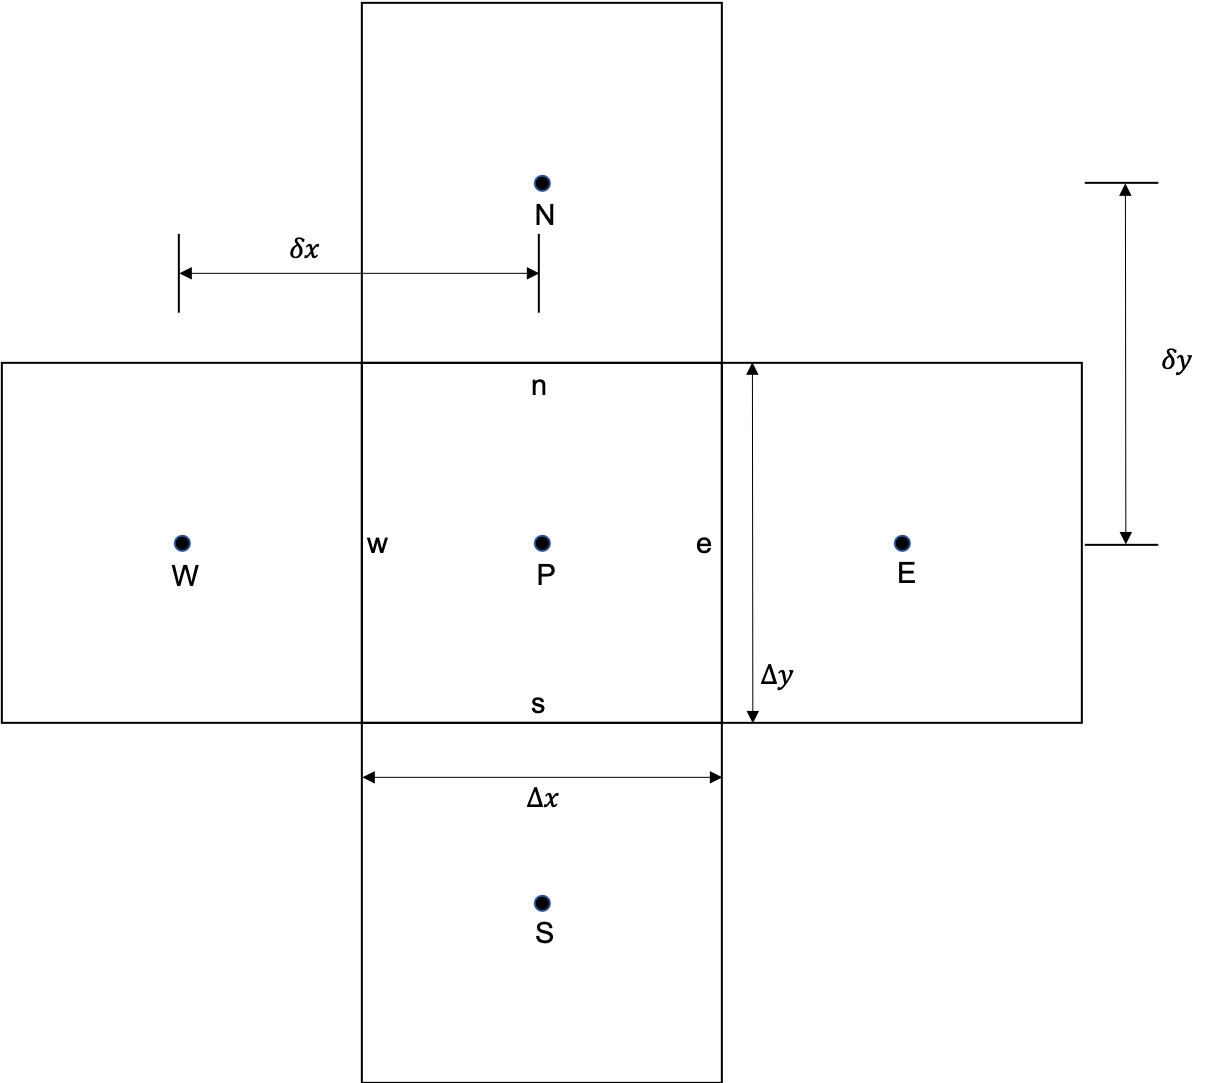
\includegraphics[width=5in]{images/chapter-4/2DFiniteVoluem.png}\\
  \caption{2-D finite volume cell}
  \label{fig:2DFiniteVolume}
\end{figure} 

\clearpage


\begin{equation}
\begin{split}
    D_{e,i}\bigg(\frac{\partial \rho_{i}}{\partial x}\bigg)_{e}\Delta y &\approx
    D_{e,i}\bigg(\frac{\rho_{E,i} - \rho_{P,i}}{\delta x}\bigg)\Delta y +
    \mathcal{O}(\Delta x),
    \\
    D_{w,i}\bigg(\frac{\partial \rho_{i}}{\partial x}\bigg)_{w}\Delta y &\approx
    D_{w,i}\bigg(\frac{\rho_{P,i} - \rho_{W,i}}{\delta x}\bigg)\Delta y + \mathcal{O}(\Delta x),
    \\
    D_{n,i}\bigg(\frac{\partial \rho_{i}}{\partial y}\bigg)_{n}\Delta x &\approx
    D_{n,i}\bigg(\frac{\rho_{N,i} - \rho_{P,i}}{\delta y}\bigg)\Delta x +
    \mathcal{O}(\Delta y),
    \\
    D_{s,i}\bigg(\frac{\partial \rho_{i}}{\partial y}\bigg)_{s}\Delta x &\approx
    D_{s,i}\bigg(\frac{\rho_{P,i} - \rho_{S,i}}{\delta y}\bigg)\Delta x +
    \mathcal{O}(\Delta y).
\end{split}
\end{equation}

\noindent Plugging these into the diffusion term in the MSR depletion equation gives,

\begin{equation}
\begin{split}
    \frac{1}{V}\int_{V}\nabla \cdot j_{i} &\approx \frac{D_{e,i}}{\Delta x}\bigg(\frac{\rho_{E,i} - \rho_{P,i}}{\delta x}\bigg) - \frac{D_{w,i}}{\Delta x}\bigg(\frac{\rho_{P,i} - \rho_{W,i}}{\delta y}\bigg) \\ \\
    &+ \frac{D_{n,i}}{\Delta y}\bigg(\frac{\rho_{N,i} - \rho_{P,i}}{\delta y}\bigg) - \frac{D_{s,i}}{\Delta y}\bigg(\frac{\rho_{P,i} - \rho_{S,i}}{\delta y}\bigg).
    \label{eq:diffusionApproximationMSRDepletion}
\end{split}
\end{equation}

\noindent Even though each of the derivative approximations for the flux across each surface where first order, the over all order for the diffusion term at point P is second. It can be shown that the approximation to the second order diffusion term used here, is equivalent to the central difference approximation to the second derivative from a finite difference scheme.

Equation \ref{eq:diffusionApproximationMSRDepletion} can be rearranged into a form which represents the coefficients for an interior node of the transition matrix. For species \textit{i} the coefficients representing diffusion are written as, 

\begin{equation}
    \frac{d \rho_{P}}{dt} = a^{D}_{E}\rho_{E} + a^{D}_{S}\rho_{S} + a^{D}_{P}\rho_{P} + a^{D}_{W}\rho_{W} + a^{D}_{N}\rho_{N},
\end{equation}

\noindent where,

\begin{equation*}
    a^{D}_{E} = \frac{D_{e}}{\Delta x \delta x}, \quad 
    a_{S} = \frac{D_{s}}{\Delta y \delta y}, \quad
    a_{W} = \frac{D_{w}}{\Delta x \delta x}, \quad
    a_{N} = \frac{D_{n}}{\Delta y \delta y},
\end{equation*}

\begin{equation*}
    a^{D}_{P} = - (a^{D}_{E} + a^{D}_{S} + a^{D}_{W} + a^{D}_{N}).
\end{equation*}

\subsubsection{Convection}
Convection-diffusion problems are difficult to numerically model because of the relative strengths each of the operators has on the species transport. These relative strengths can be illustrated by the non-dimensional Peclet number \cite{versteeg2007},

\begin{equation}
    Pe = \frac{\text{Convection}}{\text{Diffusion}} = \frac{\rho v}{D/\delta x}.
\end{equation}

\noindent As convective forces grow relative to the diffusive, the Peclet number gets larger and larger approaching infinity. On the other hand, if the diffusive forces grow at a rate larger than the convective, the Peclet number approaches zero. 

The convective transport term is more complicated and harder to deal with than the diffusion term. Diffusion has no primary direction of flow, it simply cause a species to evenly distribute through a medium through a concentration gradient. Convection on the other hand, has a primary flow direction that is driven by a pressure gradient. One of the major drawbacks of the central differencing scheme is the inability to identify flow direction. In addition to the neglect in identifying the flow direction, the central differencing scheme will cause numerical instability problems for flows with high Peclet number \cite{versteeg2007}. To combat these numerical problems and to handle flow direction, the upwind differencing scheme can be used. 

There are a number of classical differencing schemes such as, first order, power law, and QUICK, each of these will have different orders of accuracy and stability regions. Convection schemes of third order or higher can lead to undershooting or overshooting and applying boundary conditions can be problematic \cite{versteeg2007}. Because of the issues that higher order schemes can have, much development has been done into deriving a class of second-order schemes called total variation diminishing (TVD) that avoid stability and oscillation issues. TVD schemes have the property of preserving monotonicity, meaning that it must not create local extrema and the value of an existing local minimum must be non-decreasing and that of a local maximum must be non-increasing \cite{versteeg2007}. One other consequence of monotonicity preserving scheme is that the total variation of the solution should diminish or remain the same with time. 

The convection term is discretized and represented using a general second order term. First, flow is defined to be positive from cells West to East and South to North and negative in the opposite directions. For positive and negative flows, the convection operators in the x and y-directions are,

\begin{equation}
    \frac{-1}{V}\int_{V}\frac{\partial}{\partial x}(\rho_{i}v) \approx \frac{-1}{\Delta x} \big[ v_{e}\rho_{e,i} - v_{w}\rho_{w,i} \big],
\end{equation}
    
\begin{equation}
    \frac{-1}{V}\int_{V}\frac{\partial}{\partial y}(\rho_{i}v) \approx \frac{-1}{\Delta y} \big[ v_{n}\rho_{n,i} - v_{s}\rho_{s,i} \big].
\end{equation}

\noindent Plugging these in to the convective flux gives,

\begin{equation}
    \frac{-1}{V}\int_{V}\nabla \cdot \rho_{i}(r,t)\boldsymbol{v} \approx 
    \frac{1}{\Delta x} \big[ v_{w}\rho_{w,i} - v_{e}\rho_{e,i} \big] + \frac{1}{\Delta y} \big[ v_{s}\rho_{s,i} - v_{n}\rho_{n,i} \big]
\end{equation}

\noindent These equations remain constant no matter the direction of flow, the change in flow direction is taken into account with the generalized species concentration defined at each cell face. The definitions for the concentrations at each cell face are,

\begin{equation}
\begin{split}
    \text{East Face} \\ 
    \rho_{e} &= \rho_{P} + \frac{1}{2}\Psi(r_{e}^{+})(\rho_{E} - \rho_{P}), \quad v_{e}, v_{w} > 0 \\
    \rho_{e} &= \rho_{E} + \frac{1}{2}\Psi(r_{e}^{-})(\rho_{P} - \rho_{E}), \quad v_{e}, v_{w} < 0 \\
    \label{eq:eastFaceFlux}
\end{split}
\end{equation}

\vspace{-2cm}

\begin{equation}
\begin{split}
    \text{West Face} \\
    \rho_{w} &= \rho_{W} + \frac{1}{2}\Psi(r_{w}^{+})(\rho_{P} - \rho_{W}), \quad v_{e}, v_{w} > 0 \\
    \rho_{w} &= \rho_{P} + \frac{1}{2}\Psi(r_{w}^{-})(\rho_{W} - \rho_{P}), \quad v_{e}, v_{w} < 0 \\
    \label{eq:westFaceFlux}
\end{split} 
\end{equation}

\vspace{-2cm}

\begin{equation}
\begin{split}
    \text{North Face} \\ 
    \rho_{n} &= \rho_{P} + \frac{1}{2}\Psi(r_{n}^{+})(\rho_{N} - \rho_{P}), \quad v_{n}, v_{s} > 0 \\
    \rho_{n} &= \rho_{N} +
    \frac{1}{2}\Psi(r_{n}^{-})(\rho_{P} - \rho_{N}), \quad v_{n}, v_{s} < 0 \\
    \label{eq:northFaceFlux}
\end{split}
\end{equation}

\vspace{-2cm}

\begin{equation}
\begin{split}
    \text{South Face} \\
    \rho_{s} &= \rho_{S} + \frac{1}{2}\Psi(r_{s}^{+})(\rho_{P} - \rho_{S}), \quad v_{n}, v_{s} > 0 \\
    \rho_{s} &= \rho_{P} + \frac{1}{2}\Psi(r_{s}^{-})(\rho_{S} - \rho_{P}), \quad v_{n}, v_{s} < 0 
    \label{eq:southFaceFlux}
\end{split}
\end{equation}

\noindent where $\Psi$ is the flux limiter function and $r$ is the ratio of the upwind side gradient and the downwind side gradient \cite{versteeg2007}. For each cell face, the ratios for positive ($r^{+}$) and negative ($r^{-}$) flows are defined by,

\begin{equation}
    r_{e}^{+} = \bigg( \frac{\rho_{P} - \rho_{W}}{\rho_{E} - \rho_{P}}\bigg), \quad \quad r_{e}^{-} = \bigg( \frac{\rho_{EE} - \rho_{E}}{\rho_{E} - \rho_{P}}\bigg),
\end{equation}

\begin{equation}
    r_{w}^{+} = \bigg( \frac{\rho_{W} - \rho_{WW}}{\rho_{P} - \rho_{W}}\bigg), \quad \quad r_{w}^{-} = \bigg( \frac{\rho_{E} - \rho_{P}}{\rho_{P} - \rho_{W}}\bigg),
\end{equation}

\begin{equation}
    r_{n}^{+} \bigg( \frac{\rho_{P} - \rho_{S}}{\rho_{N} - \rho_{P}} \bigg), \quad \quad r_{n}^{-} = \bigg( \frac{\rho_{NN} - \rho_{N}}{\rho_{N} - \rho_{P}} \bigg),
\end{equation}

\begin{equation}
    r_{s}^{+} = \bigg( \frac{\rho_{S} - \rho_{SS}}{\rho_{P} - \rho_{S}}\bigg), \quad \quad r_{s}^{-} = \bigg(\frac{\rho_{N} - \rho_{P}}{\rho_{P} - \rho_{S}} \bigg).
\end{equation}

The criteria for a scheme to be TVD was derived by Sweby \cite{sweby1984} using the $\Psi - r$ relationship,

\begin{equation}
\begin{split}
    0 < r < 1, &\quad \Psi(r) \leq 2r \\
    r \geq 1, &\quad  \Psi (r) \leq 2.
\end{split}
\end{equation}

\noindent There are a number of flux limiters which can be applied to Equations \ref{eq:eastFaceFlux} - \ref{eq:southFaceFlux}: some of the most popular limiter functions are, Van Leer, Van Albada, Min-Mod, SUPERBEE, QUICK and UMIST. Figure \ref{fig:fluxlimiter} shows the grey shaded region for a second order scheme to be TVD, along with common flux limiter functions. In Figure \ref{fig:fluxlimiter} many of the limiter functions overlap. For the region of $r > 1$ QUICK and UMIST are the exact same and for $r > 5$ UMIST, QUICK and SUPERBEE are the same. 




TVD schemes can become unstable due to negative main coefficients and they are often reformulated in a different way to maintain numerical stability. One of the ways in which TVD schemes can be reformulated is by deferred corrections. This is an iterative method which breaks apart the convective flux coefficients into its first order upwind difference component and the second order component. The upwind differencing components will still appear in the usual matrix element however, the second order approximations are moved into a source term. The source term for step $n$ is calculated using species densities from step $n-1$. In this way the source term is differed and the convection flux is corrected. This method can be implemented both explicitly or implicitly. If the implicit formulation is used then a method such as Newton must be used to allow the solution to converge at each time step. The explicit method does not require internal iterations at each step but does require small time steps to increase the accuracy and maintain stability for the second order portion. The explicit method is utilized in Libowski. For smooth functions this formulation is second order, but reverts back to first order for discontinuous functions.  

Coefficients for the convection flux can also be rewritten in the same way that was done for the diffusion coefficients. The deferred corrections are placed in a source term coefficient. For an interior node of species \textit{i}, the transition matrix will have coefficients representing,

\clearpage

\begin{figure}[p]
  \centering
  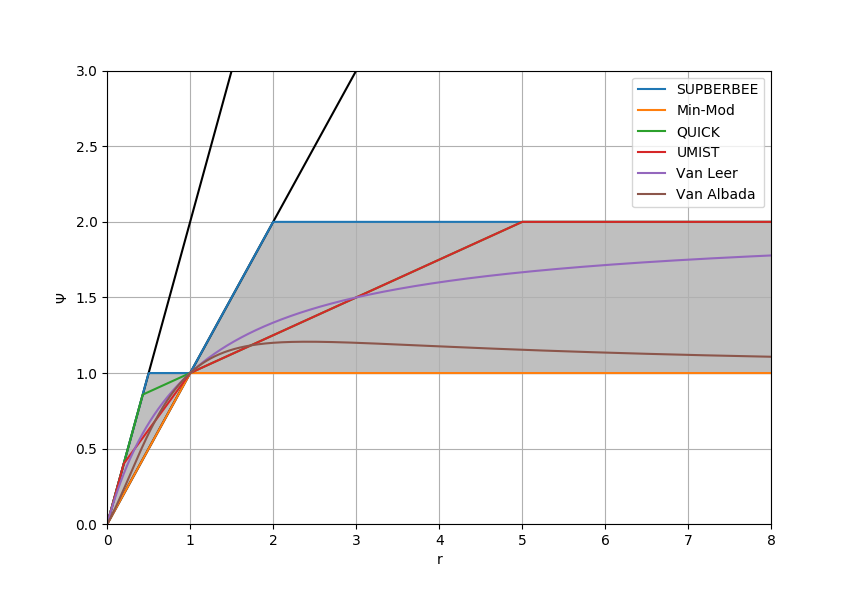
\includegraphics[width=5.5in]{images/chapter-4/CFLlimiterFunctions.png}\\
  \caption{Flux limiter functions on the $\Psi - r$ plane}
  \label{fig:fluxlimiter}
\end{figure} 

\clearpage

\begin{equation}
    \frac{d \rho_{P}}{dt} = a^{C}_{E}\rho_{E} + a^{C}_{S}\rho_{S} + a^{C}_{P}\rho_{P} + a^{C}_{W}\rho_{W} + a^{C}_{N}\rho_{N} + S^{C},
\end{equation}

\noindent where,

\begin{equation*}
    S^{C} = S_{E}^{C} + S_{S}^{C} + S_{W}^{C} + S_{N}^{C}
\end{equation*}

\begin{equation*}
\begin{split}
    a^{C}_{E} = \max\bigg(\frac{-v_{e}}{\Delta x}, 0\bigg), \quad 
    a^{C}_{S} = \max\bigg(\frac{v_{s}}{\Delta y}, 0\bigg), \quad \\
    a^{C}_{W} = \max\bigg(\frac{v_{w}}{\Delta x}, 0\bigg), \quad
    a^{C}_{N} = \max\bigg(\frac{-v_{n}}{\Delta y}, 0\bigg), \quad 
\end{split}
\end{equation*}

\begin{equation*}
    a_{P}^{C} = -(a_{E}^{C} + a_{S}^{C} + a_{W}^{C} + a_{N}^{C})
\end{equation*}

\begin{equation*}
    S^{C}_{E} = \frac{v_{e}}{2\Delta x}\bigg[(1-\alpha_{e})\Psi(r_{e}^{-}) - \alpha_{e}\Psi(r_{e}^{+})\bigg](\rho_{E} - \rho_{P}), \quad \substack{\alpha_{e} = 0, \quad v_{e} < 0\\
    \\
    \alpha_{e} = 1, \quad v_{e} > 0}
\end{equation*}

\begin{equation*}
    S^{C}_{S} = \frac{v_{s}}{2\Delta y}\bigg[(1-\alpha_{s})\Psi(r_{s}^{-}) - \alpha_{s}\Psi(r_{s}^{+})\bigg](\rho_{S} - \rho_{P}), \quad \substack{\alpha_{s} = 0, \quad v_{s} < 0\\
    \\
    \alpha_{s} = 1, \quad v_{s} > 0}
\end{equation*}

\begin{equation*}
    S^{C}_{W} = \frac{v_{w}}{2\Delta x}\bigg[(1-\alpha_{w})\Psi(r_{w}^{-}) - \alpha_{w}\Psi(r_{w}^{+})\bigg](\rho_{W} - \rho_{P}), \quad \substack{\alpha_{w} = 0, \quad v_{w} < 0\\
    \\
    \alpha_{w} = 1, \quad v_{w} > 0}
\end{equation*}

\begin{equation*}
    S^{C}_{N} = \frac{v_{n}}{2\Delta y}\bigg[(1-\alpha_{n})\Psi(r_{n}^{-}) - \alpha_{n}\Psi(r_{n}^{+})\bigg](\rho_{N} - \rho_{P}), \quad \substack{\alpha_{n} = 0, \quad v_{n} < 0\\
    \\
    \alpha_{n} = 1, \quad v_{n} > 0}
\end{equation*}



\subsection{Linear Source Terms}
Source terms considered thus far are for nuclear reactions. In this transition matrix they are the same as for traditional nuclear burnup equations and the coefficients were shown in Equations \ref{eq:diagonalCoeffsTraditionalBurnup} and \ref{eq:offdiagonalCoeffsTraditionalBurnup}. Diagonal coefficients correspond to the depletion of a species while off diagonal elements are generation terms. For species \textit{i} is interior cell \textit{P} the coefficients of the transition matrix for linear sources are,

\begin{equation}
    \frac{d \rho_{P,i}}{dt} = a_{P,i}^{LS}\rho_{P,i} + \sum_{j=1, j \neq i}^{N}a_{P,j}^{LS}\rho_{P, j} + \sum S^{C}_{i}
\end{equation}


\noindent These source terms will also include the deferred corrections from a second order upwind flux approximation represented as constant source terms. 

Nuclear reaction rates are calculated in such a way to preserve reaction rates. This is done by integrating over all neutron energies and the volume of the cell. Over a single burn up calculation step all cross sections and the scalar neutron flux is assumed to be constant. Using volume average operators and the multigroup approximation, the neutron flux and microscopic cross section is collapsed into single values for each depletion zone \cite{aarnoThesis}:

\begin{equation}
    \sigma_{k,j} = \frac{\int_{V}\int_{0}^{\infty}\sigma_{k,j}(r,E)\phi(r,E) dEdV}{\int_{V}\int_{0}^{\infty}\phi(r,E) dEdV},
\end{equation}

\begin{equation}
    \phi = \frac{1}{V}\int_{V}\int_{0}^{\infty}\phi(r,E)dEdV.
\end{equation}

\noindent Source terms for nuclear reactions are not calculated inside of Libowski. Thus, for nuclear reactions, an external source must provide the cross sections, neutron flux and decay constants already calculated in the correct manner. These reactions are added to the transition matrix and are expressed as:

\begin{equation}
    a^{LS}_{P,i} = \lambda_{i} + \overline{\phi}\sum_{k=1}^{K} \overline{\sigma}_{k,i}, \quad 
    a^{LS}_{P,j} = \frac{M_{i}}{M_{j}}\bigg(b_{j\rightarrow i}\lambda_{j} +
    \sum_{k=1}^{K}\gamma_{j\rightarrow i,k}\overline{\sigma}_{k,j}(r)\overline{\phi} \bigg).
\end{equation}

Both of the mass transport models were implemented by added linear coefficients to the transition matrix. If a single species has the ability to transport from the liquid or the wall or gas phase then that species is duplicated three times. In the cases of Xe, if Xe is allowed to transport to the gas bubbles or the wall then Xe will have three individual species \textit{XeLiq}, \textit{XeGas} and \textit{XeWall}. Xe generated in the liquid from fission would be allowed to transport to the gas bubbles or the wall via terms in the transition matrix which are calculated using the mass transfer models. In addition to the mass transfer coefficient, scalar variables such as temperature, interfacial area, gas void fraction and Henry's Law coefficients are required to compute the transition coefficient. 

For species $i$ the following relations represent the mass transfer model for cases when the species exist on the wall or in the liquid:

\begin{equation}
    \frac{d\rho_{i, \text{wall}}}{dt} = \frac{kA}{V}(\rho_{i, \text{liquid}} - \rho_{i,\text{wall}}) \quad \quad \text{Species exist on wall},
\end{equation}

\begin{equation}
    \frac{d\rho_{i, \text{liquid}}}{dt} = \frac{kA}{V}(\rho_{i,\text{wall}} - \rho_{i,\text{liquid}}) \quad \quad \text{Species exist in liquid},
\end{equation}

\noindent where $A$ is the wall area [m$^2$], $V$ is the cell volume [m$^3$] and $k$ is the mass transfer coefficient [m/s]. It is often to express $A/V$ as the interfacial area concentration.The mass transfer coefficient and wall area concentration have to be set by the user when creating the model. In the transition matrix, these coefficients are expressed as:

\begin{equation}
    a^{LS}_{P,i, \text{wall}} = -\frac{kA}{V}, \quad 
    a^{LS}_{P,j, \text{liquid}} = \frac{kA}{V}.
\end{equation}

\begin{equation}
    a^{LS}_{P,i, \text{liquid}} = -\frac{kA}{V}, \quad 
    a^{LS}_{P,j, \text{wall}} = \frac{kA}{V}.
\end{equation}

\noindent In some situations an infinite sink approximation may be appropriate \cite{kedl1972}. This assumes that the species build up on the wall will not influence the mass transfer rate to the wall, reducing the model to: 

\begin{equation}
    \frac{d\rho_{i, \text{wall}}}{dt} = \frac{kA}{V}\rho_{i,\text{liquid}},
\end{equation}

\begin{equation}
    \frac{d\rho_{i, \text{liquid}}}{dt} = -\frac{kA}{V}\rho_{i,\text{liquid}}.
\end{equation}

Gas transport is implemented in a similar way to wall deposition however, the transition coefficient is more complex. Starting with the flux across the bubble interface:

\begin{equation}
    j = k_{l}(\rho^{l}_{*} - \rho^{l}_{\text{bulk}}).
\end{equation}

\noindent where $\rho^{l}_{*}$ is calculated using the gas phase concentration and $\rho^{l}_{\text{bulk}}$ is the liquid phase concentration. Starting with Henry's law for ideal systems, the concentration of gas species $i$ dissolved in the liquid phase is calculated to be:

\begin{equation}
    C_{i} = H_{i}P_{i},
\end{equation}

\noindent where $H_{i}$ is the Henry's law coefficient [kg/Pa/m$^3$] and $P_{i}$ is the partial pressure [Pa] of species $i$. A gas phase species partial pressure is required to calculate the amount of gas dissolved in the liquid. For an ideal gas, the partial pressure can be related to the gas phase mass density starting with the ideal gas law:

\begin{equation}
    P = \frac{nRT}{V}.
\end{equation}

\noindent where $n$ is moles of gas [mol], R is ideal gas constant [m$^3$Pa/mole/K], and T is temperature [K]. Dalton's law says that the total in the gas phase is equal to a summation of the partial pressures of each individual gas component:

\begin{equation}
    P_{\text{total}} = P_{1} + P_{2} + P_{3} ... = \sum_{i=1}^{N} P_{i}, 
\end{equation}

\noindent where partial pressure $P_{i} = P_{\text{total}}x_{i}$ and $x_{i}$ is the mole fraction of species $i$ in the gas phase. Combining Dalton's law and the ideal gas law gives a relation for the partial pressure:

\begin{equation}
    P_{i} = \frac{nRT}{V}\frac{n_{i}}{n} = \frac{n_{i}RT}{V}. 
\end{equation}

\noindent In Libowski, species concentrations are solved for mass density in the entire cell volume however, volume in the ideal gas law is for the gas phase. These two volumes are related using the gas void fraction, $V_{\text{gas}} = V_{\text{cell}}\alpha_{\text{gas}}$. Using the volume relation and the molar mass $MM_{i}$ [g/mol] of the gas, the partial pressure of gas $i$ in terms of mass density [kg/m$^3$] is:

\begin{equation}
    P_{i} = \frac{1000RT}{\alpha_{\text{gas}}MM_{i}}\rho_{i}^{g}. 
\end{equation}

\noindent Plugging this relation into Henry's law gives the equilibrium concentration of gas dissolved in the liquid in terms of mass density in the gas phase:

\begin{equation}
    \rho_{*,i}^{l} = \frac{1000H_{i}RT}{\alpha_{\text{gas}}MM_{i}}\rho_{i}^{g}
\end{equation}

\noindent For species $i$ the following relations represent the mass transfer model for cases when the species exist in the gas bubbles or the liquid:

\begin{equation}
    \frac{d\rho_{i, \text{gas}}}{dt} = \frac{kA}{V}\bigg(\rho_{i,\text{liquid}} - \frac{1000H_{i}RT}{\alpha_{\text{gas}}MM_{i}}\rho_{i, \text{gas}}\bigg) \quad \quad \text{Species exist in gas},
\end{equation}

\begin{equation}
    \frac{d\rho_{i, \text{liquid}}}{dt} = \frac{kA}{V}\bigg(\frac{1000H_{i}RT}{\alpha_{\text{gas}}MM_{i}}\rho_{i, \text{gas}} - \rho_{i,\text{liquid}}\bigg) \quad \quad \text{Species exist in liquid},
\end{equation}

\noindent where $k$ is the mass transfer coefficient [m/s] and $A$ is the interfacial area of the gas phase [m$^2$]. Again, the interfacial area concentration $A/V$ is set by the user. In the transition matrix, these coefficients are expressed as:

\begin{equation}
    a^{LS}_{P,i, \text{gas}} = -\frac{kA}{V}\frac{1000H_{i}RT}{\alpha_{\text{gas}}MM_{i}}, \quad 
    a^{LS}_{P,j, \text{liquid}} = \frac{kA}{V}.
\end{equation}

\begin{equation}
    a^{LS}_{P,i, \text{liquid}} = -\frac{kA}{V}, \quad 
    a^{LS}_{P,j, \text{gas}} = \frac{kA}{V}\frac{1000H_{i}RT}{\alpha_{\text{gas}}MM_{i}}.
\end{equation}

\subsection{Treatment of Boundary Conditions}
Dirichlet and Neumann boundary conditions can be easily implemented by the use of "ghost" cells. Ghost cells are cell which are placed outside the boundary of our domain and will allow for a scalar value or the derivative of a scalar value to be set at the boundary of the domain. For example, take a 2-D example of the species transport equation. The differential equation for node $P$ would be,

\begin{equation}
    \frac{d\rho}{dt} = a_{E}\rho_{E} + a_{S}\rho_{S} + a_{P}\rho_{P} + a_{N}\rho_{N} + a_{W}\rho_{W} + S
\end{equation}

\noindent If $P$ was at the East boundary then a Dirichlet boundary condition means that the value at the cell boundary is fixed $(\rho_{e} = \rho_{b,r}$). Because there is a ghost cell to the East of cell $P$, the boundary value can be implemented using a difference across the two cells,

\begin{equation}
    \rho_{e} = \rho_{b} \approx \frac{\rho_{P} + \rho_{E}}{2}.
\end{equation}

\noindent The species concentration for the East cell is solved for and plugged back in to the differential equation to yield new coefficients for the matrix elements. This same method is used for the top, bottom, left, right and the corners. Let the subscript \textit{b} denote a boundary condition value and let \textit{r}, \textit{l}, \textit{t} and \textit{b} denote the right, left, top and bottom boundaries. Table \ref{tab:dirichletBoundaries} shows the modified coefficients for Dirichlet boundary conditions. 

Neumann boundary conditions are applied in a similar way by approximating the derivative at the boundary using a second order central difference approximation at the boundary. For the bottom boundary this leads to,

\begin{equation}
    \rho_{b}' \approx \frac{\rho_{P} - \rho_{S}}{\delta y}.
\end{equation}

\noindent The concentration in the south boundary cell is solved for and plugged back into the differential equation. A similar process is done for the top, left, right and corners. The results are shown in Table \ref{tab:newmannBoundaries} for the modified coefficients. A mixture of both of these boundary conditions can be used for each side, although special care needs to be taken with the corners if the boundary conditions are mixed. 

Periodic boundary conditions are applied on either the top and bottom or the left and right. This type of boundary condition can be thought of as folding the rectangular domain 

\clearpage

\begin{table}[p]
    \caption{\label{tab:dirichletBoundaries} Modified Coefficients for Dirichlet Boundaries}
    \centering
    \begin{tabular}{c|c|c|c|c|c|c}
    \hline
    \textbf{Boundary location} & \textbf{$a_{E}^{*}$} & \textbf{$a_{S}^{*}$} & \textbf{$a_{P}^{*}$} & \textbf{$a_{N}^{*}$} & \textbf{$a_{W}^{*}$} & \textbf{$S^{*}$} \\ [0.5ex]
    \hline
    \hline
    Bottom & $a_{E}$ & $0$ & $a_{P} - a_{S}$ & $a_{N}$ & $a_{W}$ & $S + 2a_{S}\rho_{bb}$\\ \hline
    Top & $a_{E}$ & $a_{S}$ & $a_{P} - a_{N}$ & $0$ & $a_{W}$ & $S + 2a_{N}\rho_{bt}$ \\ \hline 
    Left & $a_{E}$ & $a_{S}$ & $a_{P} - a_{W}$ & $a_{N}$ & $0$ & $S + 2a_{W}\rho_{bl}$  \\ \hline
    Right & $0$ & $a_{S}$ & $a_{P} - a_{E}$ & $a_{N}$ & $a_{W}$ & $S + 2a_{E}\rho_{br}$  \\ \hline
    Bottom left corner & $a_{E}$ & $0$ & $a_{P} - a_{S} - a_{W}$ & $a_{N}$ & $0$ & $S + 2a_{S}\rho_{bb} + 2a_{W}\rho_{bl}$ \\ \hline
    Bottom right corner & $0$ & $0$ & $a_{P} - a_{S} - a_{E}$ & $a_{N}$ & $a_{w}$ & $S + 2a_{S}\rho_{bb} + 2a_{E}\rho_{br}$ \\ \hline
    Top left corner & $a_{E}$ & $a_{S}$ & $a_{P} - a_{N} - a_{W}$ & $0$ & $0$ & $S + 2a_{N}\rho_{bt} + 2a_{W}\rho_{bl}$ \\ \hline
    Top right corner & $0$ & $a_{S}$ & $a_{P} - a_{N} - a_{E}$ & $0$ & $a_{W}$ & $S + 2a_{N}\rho_{bt} + 2a_{E}\rho_{br}$ \\ \hline
    \end{tabular}
\end{table}

\clearpage

\begin{table}[p]
    \caption{\label{tab:newmannBoundaries} Modified Coefficients for Newmann Boundaries}
    \centering
    \begin{tabular}{c|c|c|c|c|c|c}
    \hline
    \textbf{Boundary location} & \textbf{$a_{E}^{*}$} & \textbf{$a_{S}^{*}$} & \textbf{$a_{P}^{*}$} & \textbf{$a_{N}^{*}$} & \textbf{$a_{W}^{*}$} & \textbf{$S^{*}$} \\ [0.5ex]
    \hline
    \hline
    Bottom & $a_{E}$ & $0$ & $a_{P} + a_{S}$ & $a_{N}$ & $a_{W}$ & $S - a_{S}\rho_{bb}'\delta y$\\ \hline
    Top & $a_{E}$ & $a_{S}$ & $a_{P} + a_{N}$ & $0$ & $a_{W}$ & $S - a_{N}\rho_{bt}'\delta y$ \\ \hline 
    Left & $a_{E}$ & $a_{S}$ & $a_{P} + a_{W}$ & $a_{N}$ & $0$ & $S - a_{W}\rho_{bl}'\delta x$  \\ \hline
    Right & $0$ & $a_{S}$ & $a_{P} + a_{E}$ & $a_{N}$ & $a_{W}$ & $S - a_{E}\rho_{br}'\delta x$  \\ \hline
    Bottom left corner & $a_{E}$ & $0$ & $a_{P} + a_{S} + a_{W}$ & $a_{N}$ & $0$ & $S - a_{S}\rho_{bb}'\delta y - a_{W}\rho_{bl}'\delta x$ \\ \hline
    Bottom right corner & $0$ & $0$ & $a_{P} + a_{S} + a_{E}$ & $a_{N}$ & $a_{w}$ & $S - a_{S}\rho_{bb}'\delta y - a_{E}\rho_{br}'\delta x$ \\ \hline
    Top left corner & $a_{E}$ & $a_{S}$ & $a_{P} + a_{N} + a_{W}$ & $0$ & $0$ & $S - a_{N}\rho_{bt}'\delta y - a_{W}\rho_{bl}'\delta x$ \\ \hline
    Top right corner & $0$ & $a_{S}$ & $a_{P} + a_{N} + a_{E}$ & $0$ & $a_{W}$ & $S - a_{N}\rho_{bt}'\delta y - a_{E}\rho_{br}'\delta x$ \\ \hline
    \end{tabular}
\end{table}

\clearpage

\noindent creating a cylinder. These are implemented by pointing the cell at one boundary next to the cell at the opposite side. For example, if periodic boundary conditions are applied on the top and bottom and the flow is positive, then what comes out the top enters at the bottom. In this way, flow loops can be modeled.


\subsection{Application of Matrix Exponential Solvers}
Five different matrix exponential solver are implemented in Libowski with the added ability to use the Krylov subspace approximation. Each of these methods were discussed in Chapter \ref{ch:matrixEXPMethods} and algorithms are presented in this section. These methods include three based on Cauchys integral formula and two based on Pad\'e's approximation with scaling and squaring. Because of the  various magnitudes of the transition matrix coefficients, a direct solver is used to solve the linear systems \cite{pusa2013}. The direct solver is Eigens sparse LU decomposition which is based on the SuperLU library \cite{eigen} \cite{superlu99}. Each of the algorithms listed in this thesis are shown in Appendix \ref{appen:matexpalg}.

\subsubsection{CRAM}
The biggest problem with using CRAM is obtaining the coefficients for the partial fraction decomposition. These coefficients for order 14 and 16 can be found in Reference \cite{pusa2011}, only order 16 is implemented in Libowski. As discussed earlier for Cauchy method of order $N$, $N/2$ number of complex linear systems need to be solved. The general algorithm for a method based on contour integrals in partial fraction decomposition form is shown in Algorithm \ref{alg:cauchy}. Both the Parabolic and Hyperbolic methods used this same algorithm but with different poles and residues. It should be noted that notation for the residues where changed from $c_{k}$ to $\alpha_{k}$ and the residues from $z_{k}$ to $\theta_{k}$. For complex matrices and scalars $\alpha$ and $\theta$ would need to be the same size as the approximation order. Real valued matrices and scalars require half of these coefficients. Because all the matrices here are real, $\alpha$ and $\theta$ are all of size $N/2$. 




\subsubsection{Parabolic and Hyperbolic}
Solutions with the parabolic and hyperbolic contours use Algorithm \ref{alg:cauchy} but with different poles and residues. While methods for evaluating the coefficients for CRAM take a long time and need to be precalculated, the poles and residues for contour functions can be computed when the solver is initialized. Calculating the coefficients requires the contour function ($\phi$), the function derivative ($\phi'$) and the order of the approximation ($N$) Algorithms \ref{alg:parabolicCoeffs} and \ref{alg:hyperbolicCoeffs} in Appendix \ref{appen:matexpalg} show the functions computing the arrays for $\alpha$ and $\theta$ with parabolic and hyperbolic contours. While any order is possible, the default order in Libowski is 32. 

\subsubsection{Parallelization of Cauchy Solvers}
As mentioned before, for a given order $N$ of the Cauchy solvers $N/2$ linear systems need to be solved. Each of these systems are independent and can be performed separately. Paralelization takes two general forms: shared and distributed memory. Shared memory archetypes involve using multicore CPUs which have access to the same shared memory. Because of this; all processors have access to the same set of variables and can modify them individually. Distributed memory works by connecting multiple CPUs over a network and having each computer solve a portion of the problem. In this case; each computer has its own copy of the variables required to solve its portion of the problem. Libraries exist which allow programmers the ability to parallelize their code on a high level for each of these two architectures. Open multiprocessing (OpenMP) is used for shared memory and message massing interface (MPI) for distributed memory \cite{openmp} \cite{mpi}. In general OpenMP is easier to implement but less flexible because of the memory requirement. This issue with MPI is that using it on a shared memory device will unnecessarily increase the memory consumption. Because of its inherent flexibility MPI is utilized in parallizing the Cauchy solver in Libowski. 

\subsubsection{Pad\'e - Method 1}
The first method bast on the Pad\'e approximation was developed by Nicholas J. Higham and can be found in Reference \cite{higham2005}. Higham developed this algorithm in a similar manner which was done before by Moler and Van Loan \cite{moler2003} by choosing the optimal number of matrix scalings required for the Pad\'e of a certain order. Higham noted that the backward error analysis done by Moler and Van Loan was simple and elegant, however not sharp. Instead of only developing an algorithm based on a numerical error bound, Highman also considered computational cost. The resulting algorithm developed by Highman can be found in Reference \cite{higham2005} and the reader should refer to Highman's paper for further detail in its development. Algorithm \ref{alg:method1} is the algorithm that was developed in the paper, and shows its implementation in Libowski. From now it shall be referred to as Pad\'e Method 1. Pad\'e Method's 1 and 2 both rely on functions that are shown in Appendix \ref{appen:matexpalg}. Unlike methods based on contour functions, the Pad\'e method directly computes the matrix exponential. 

\subsubsection{Pad\'e - Method 2}
The second Pad\'e method is a modification of the first Pad\'e method that addresses the weakness in overscaling. Overscaling occurs when a large matrix norm causes a larger than necessary $\alpha$ to be used, leading to decreased accuracy \cite{higham2009}. Al-Mohy and Higham developed this algorithm by inroducing a new sharper truncation error bound, which is likely to help correct the overscaling problem. More information on the new algorithm can be found in Referenence \cite{higham2009}. Algorithm 6.1 from said reference is implemented in Libowski and is shown in Algorithm \ref{alg:method2}. There are two helper functions that are used in Algorithm \ref{alg:method2}, these function are defined Appendix \ref{appen:matexpalg} along with Algorithm \ref{alg:method2}. 


\subsubsection{Taylor}
The Taylor algorithms implemented in Libowski was taken from Reference \cite{higham2011} for computing $\boldsymbol{F} \approx e^{\boldsymbol{A}t}\boldsymbol{B}$ over a single step, where $\boldsymbol{A} \in \mathbb{C}^{n\times n}$ and $\boldsymbol{B} \in \mathbb{C}^{n\times n_{0}}$. Unlike the Pad\'e methods, the Taylor algorithm does not require the need for linear solves. This was done in an attempt to reduce the computational cost. Three key ideas were employed when developing this algorithm:

\begin{enumerate}
    \item Careful choice of the Taylor series order and scaling parameter, exploiting estimates of $||t{\boldsymbol{A}}^{p}||^{p}$, to keep the backward error suitably bounded while minimizing the computational cost.
    \item Shifting, and optional balancing, to reduce the norm of $\boldsymbol{A}t$.
    \item Premature termination of the truncated Taylor series evaluations.
\end{enumerate}


One of the major components of this algorithm is in picking the optimal Taylor order and scaling parameter. This is accomplished by minimizing the computational cost while choosing the appropriate scaling and squaring parameter to obtain a backwards error below a minimal tolerance. For this algorithm, the parameters function accomplishes this and is shown in Algorithm \ref{alg:taylor_parameters}. This algorithm requires 2 additional parameters $p_{\text{max}}$ and $m_{\text{max}}$, where $m_{\text{max}}$ is the maximum order of the Taylor series. The first parameter $p_{\text{max}}$ is the largest integer such that $p(p - 1) \leq m_{\text{max}} + 1$. For values of $m$ up to 100, $p_{\text{max}}$ are tabulated in table \ref{tab:pmax_mmax_values}. Reference \cite{higham2011} notes that as $m_{\text{max}}$ increases the overall cost of the algorithm decreases however, large values of $m$ can lead to numerical instability. The default parameters, which were recommended by Al-Mohy et al., are $p_{\text{max}} = 8$ and $m_{\text{max}} = 55$.  

 